\documentclass[a4paper,12pt,titlepage]{article}
\usepackage[pdftex]{graphicx}
\usepackage[headheight=15pt]{geometry}

\usepackage{fancyhdr}
\pagestyle{fancy}
\lhead{Exercises}
\chead{}
\rhead{InaSAFE}

\usepackage[english]{babel}									
\usepackage[utf8]{inputenc}	

\usepackage{array}
\usepackage{colortbl}

\usepackage[section]{placeins}
\usepackage{float}

%PDF hyperlinks
\usepackage[colorlinks=true,linkcolor=orange,citecolor=blue,bookmarksopen=true,bookmarksnumbered=true,pdfstartpage=1]{hyperref}
\hypersetup{
	pdftitle={Using InaSAFE for disaster impact assessment},
	pdfauthor={Michael Wagner},
	pdfsubject={InaSAFE, impact assessment},
	pdfkeywords={GIS, QGIS, InaSAFE, impact assessment}
}

\usepackage[nonumberlist,nopostdot]{glossaries}
% Set width of the abbreviation column
\setglossarystyle{alttree}
\glssetwidest{SWIO-RAFI-XX}
%
\makeglossaries
\loadglsentries{abbr}
\setacronymstyle{long-short}

\usepackage{color}
\definecolor{orange}{rgb}{1,.5,0}


\title{Exercises: Using InsSAFE for disaster impact assessment}
\author{Michael Wagner (mwagner@allspatial.info)}
\date{July 13, 2016}     													

\clubpenalty=4500																
\widowpenalty=10000								
\linespread{1.3}

%%-------------------------Document begins--------------------------------------------
\begin{document}             										
\maketitle                   									

\tableofcontents
\listoffigures
\newpage
\printglossary[type=\acronymtype,title={List of Abbreviations}]
\newpage

\section{Introduction}

InaSAFE is plugin for QGIS to perform disaster impact assessments. It facilitates analyses such as \textit{Which structures and to what level are affected by a flood}. Each layer/dataset used in InaSAFE falls in one of the following three categories:

\begin{itemize}
	\item Hazard
	\item Exposure
	\item Aggregation 
\end{itemize}

The user has to assign one of these categories to each datasets to be used in an InaSAFE analysis. This is done by using the \textit{Keywords Creation Wizard} covered at a later stage during this exercise. Once the categories have been assigned InaSAFE facilitates impact assessment analyses by performing on a single mouse-click what otherwise would require numerous steps using the standard GIS tools available.

InaSAFE was initially developed by the Indonesian National Disaster Management Agency (BNPB), the Australian Government and the World Bank's \gls{gfdrr}. To date it has a very active user and developer community.

Download and install the InaSAFE plugin trough the \textit{Manage and Install Plugins} dialog (menu \textit{Plugins}). Enter InaSAFE in the search field and install the plugin (Figure \ref{fig:install_inasafe})

\begin{figure}[htb]
	\centering
	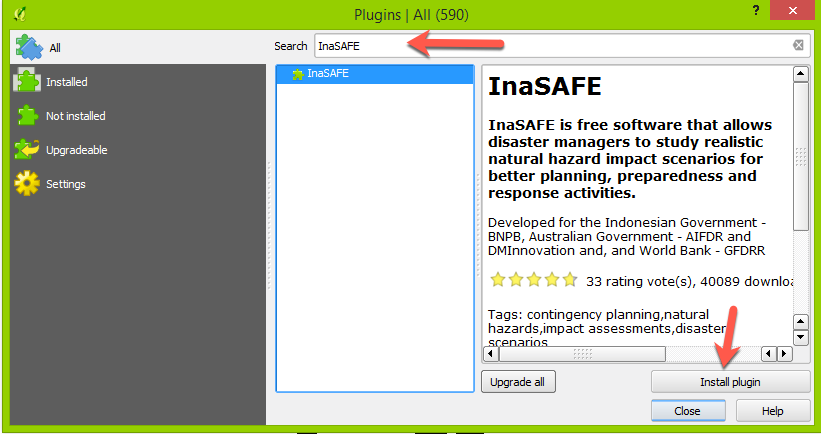
\includegraphics[width=12cm]{Images/install_inasafe.png}
	\caption{Installing InaSAFE}\label{fig:install_inasafe}
\end{figure}

\section{Preparing the hazard data}

\subsection{Loading the DEM}

From the \textit{Data/DEM} folder load the the \gls{dem} for Mahe (\textit{Mahe\_DEM.tif}). The \gls{dem} is a raster datasets and hence, needs to be loaded through the \textit{Add Raster Layer} tool of QGIS. The \gls{dem} was generated from \gls{lidar} data and reflects the elevation of the terrain above mean sea level. QGIS will automatically assign an appropriate style to visualise the elevation range of the \gls{dem} (Figure \ref{fig:dem}). Be aware that the \gls{dem} reflects the situation from 2011. Any landfill or excavation work done since then is of course not covered.

\begin{figure}[htb]
\centering
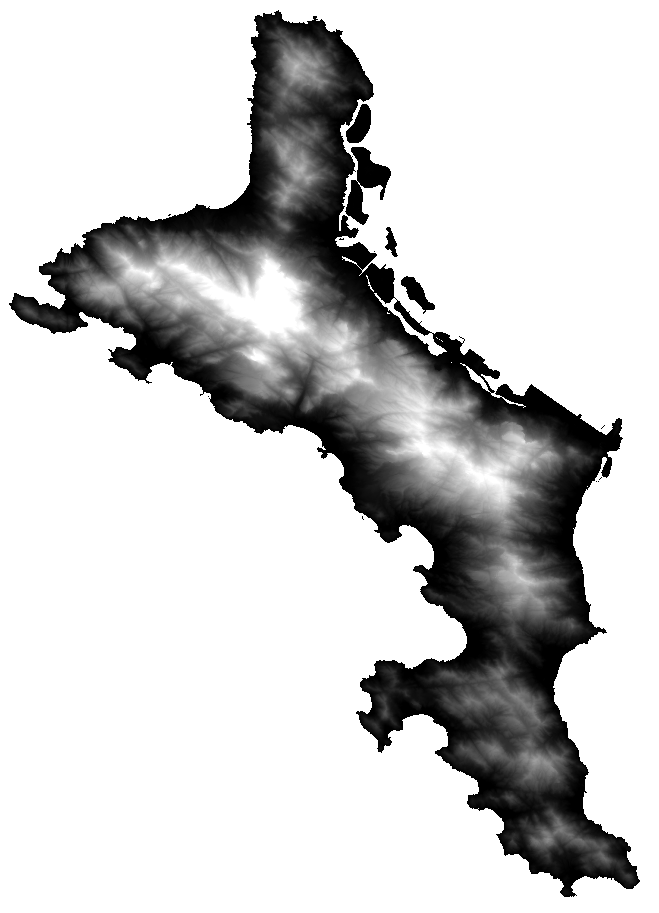
\includegraphics[width=5cm]{Images/dem.png}
\caption{DEM of Mahe}\label{fig:dem}
\end{figure}

You can use the \textit{Identify Features} tool of QGIS to get information about the individual heights in the \gls{dem}. Activate the tool and click somewhere in the \gls{dem}. The way the \gls{dem} is currently styled makes it hard to get a good idea of the terrain's shape. A much better way to visualise that is a so called hillshade image. Select the \textit{Hillshade} tool from the \textit{Raster:Terrain Analysis} menu. Leave the settings as shown in Figure \ref{fig:hillshade} and click OK. Depending on your computer's performance generating the hillshade image might take a few seconds.

\begin{figure}[htb]
	\centering
	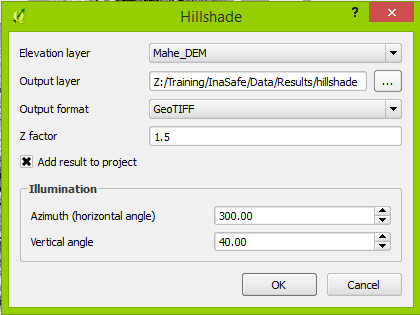
\includegraphics[width=8cm]{Images/hillshade.png}
	\caption{Settings for hillshade image}\label{fig:hillshade}
\end{figure}

Experiment with the z-factor and illumination settings and create a few hillshade images to see how these settings are reflected. The z-factor can be used to visualise even small differences in elevation and is in a way an ``exaggeration-factor''.

\subsection{Creating the inundation layer}

Let's assume the sea level would rise 6m as a result of a Tsunami for example. You will now create an inundation map based on that assumption. From the mathematical point of view you will subtract the current terrain elevations from an assumed 6m-plane. Open the \textit{Raster Calculator} from the \textit{Raster} menu. The \textit{Raster Calculator} will automatically list all raster bands it currently finds in the table of contents. In the \textit{Raster calculator expression} field type ``6-'' and then double-click the \textit{Mahe\_DEM@1} layer to add it to the expression field. Leave all other settings as they are and click OK (Figure \ref{fig:inundation1}).

\begin{figure}[htb]
	\centering
	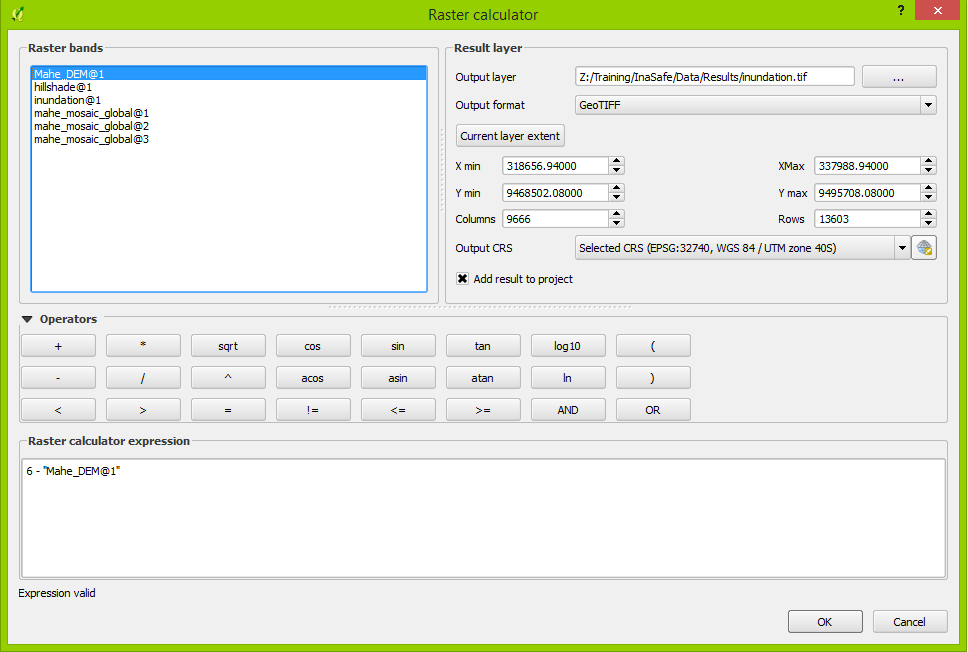
\includegraphics[width=8cm]{Images/inundation1.png}
	\caption{Raster Calculator settings}\label{fig:inundation1}
\end{figure}

The result is a raster map with positive heights for all inundated areas and negative heights for those not inundated. Keep in mind that this is a simplified approach. If you had a terrain situation as shown in Figure \ref{fig:inundation2} the sea water would never reach the B-section. However, your current calculation would show that area as inundated.

\begin{figure}[htb]
	\centering
	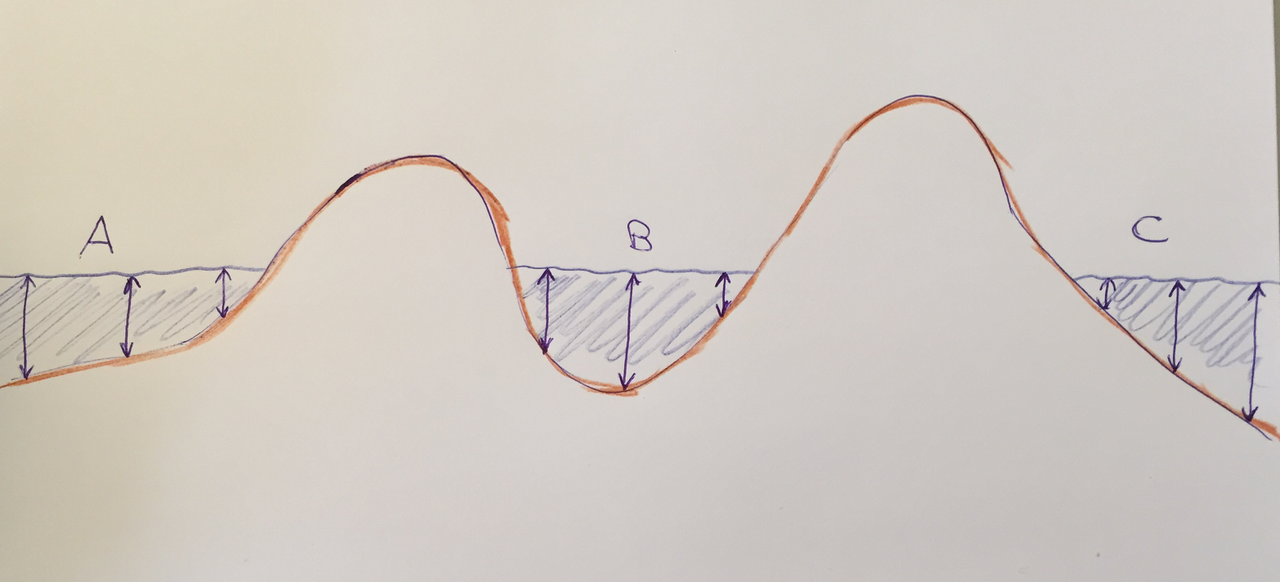
\includegraphics[width=8cm]{Images/inundation2.png}
	\caption{Simplified calculation approach}\label{fig:inundation2}
\end{figure}

For (much) faster analyses with InaSAFE you should reduce the resolution of the inundation layer to 50\%. The current resolution resulting from the original \gls{dem} is 2m/pixel. You should reduce it to 4m/pixel. You can use the \textit{Warp} tool from the \textit{Raster:Projections} menu. Use the settings as shown in Figure \ref{fig:warp}.

\begin{figure}[htb]
	\centering
	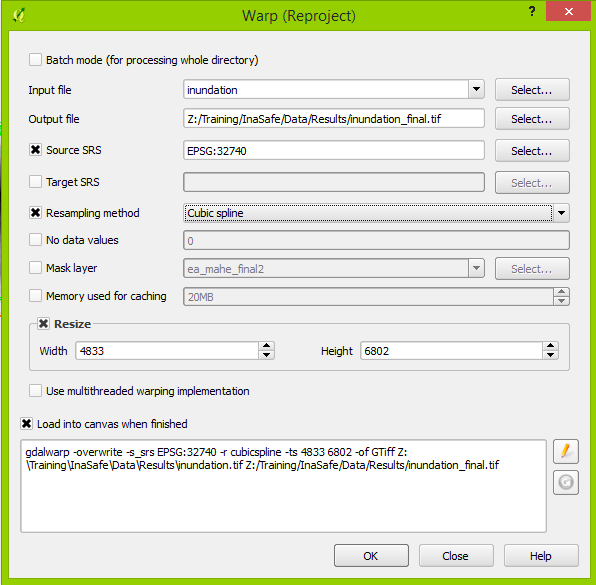
\includegraphics[width=8cm]{Images/warp.png}
	\caption{Resampling the inundation raster}\label{fig:warp}
\end{figure}


\section{Preparing the exposure data}

Load the \textit{road} and \textit{building} layers from the \textit{Data/Shapefiles} folder into QGIS. InaSAFE supports categorising the buildings and roads by type in the impact assessment results. Both layers need to have one attribute that represents their type. For buildings these types are supported by InaSAFE:

\begin{itemize}
	\item Residential
	\item Education
	\item Health
	\item Transport
	\item Place of Worship
	\item Government
	\item Commercial
	\item Recreation
	\item Public Facility
	\item Other
\end{itemize} 

For roads the types as follows are supported:

\begin{itemize}
	\item Motorway
	\item Primary
	\item Secondary
	\item Local
	\item Path
	\item Other
\end{itemize}

The \textit{road} layer has categories already assigned (attribute \textit{CATEGORY}) while the \textit{building} layer does not. In the \textit{Data/Shapefiles} folder you will find a file \textit{road\_categories.csv} with a description of the categories. For the \textit{building} layer you have to populate the categories yourself. Add a new column of type \textit{integer} to the layer and name it \textit{TYPE}. Define a number for each of the ten building types supported by InaSAFE as shown above. Health care and education relating buildings you can identify using two existing layers \textit{medical\_facility} and \textit{school} in the \textit{Data/Shapefiles} folder. These layers have point geometry but you can use a spatial query to relate them with the original \textit{building} layer and assign the building features the numeric codes you defined for the \textit{Health} and \textit{Education} categories. This approach will give you categories for very few buildings only. To the remaining ones you could randomly assign one of the other eight categories using the same methodology you used in the previous workshop to assign dates to the Dengue cases. At the end of this exercise each building should have a category/type assigned.

\section{Preparing the aggregation layer}

Load the \textit{district} layer from the \textit{Data/Shapefiles} folder into QGIS. It will allow you to aggregate the impact assessment results by district. No other preparation is required for the aggregation layer.

\section{Assigning keywords}

You now have to assign categories to the exposure, hazard and aggregation data so that InaSAFE knows what role the datasets have in the impact analysis. 

\subsection{Exposure layers}

Select the \textit{building} layer in the table of contents and click the \textit{Keyword Creation Wizard} button on the InaSAFE toolbar. Select \textit{Exposure} as the keyword (Figure \ref{fig:keyword1}). In the next step select \textit{Structure}. Click \textit{Next} twice and select \textit{TYPE} as the attribute containing the classes of structure/building (Figure \ref{fig:keyword3}).

\begin{figure}[htb]
	\centering
	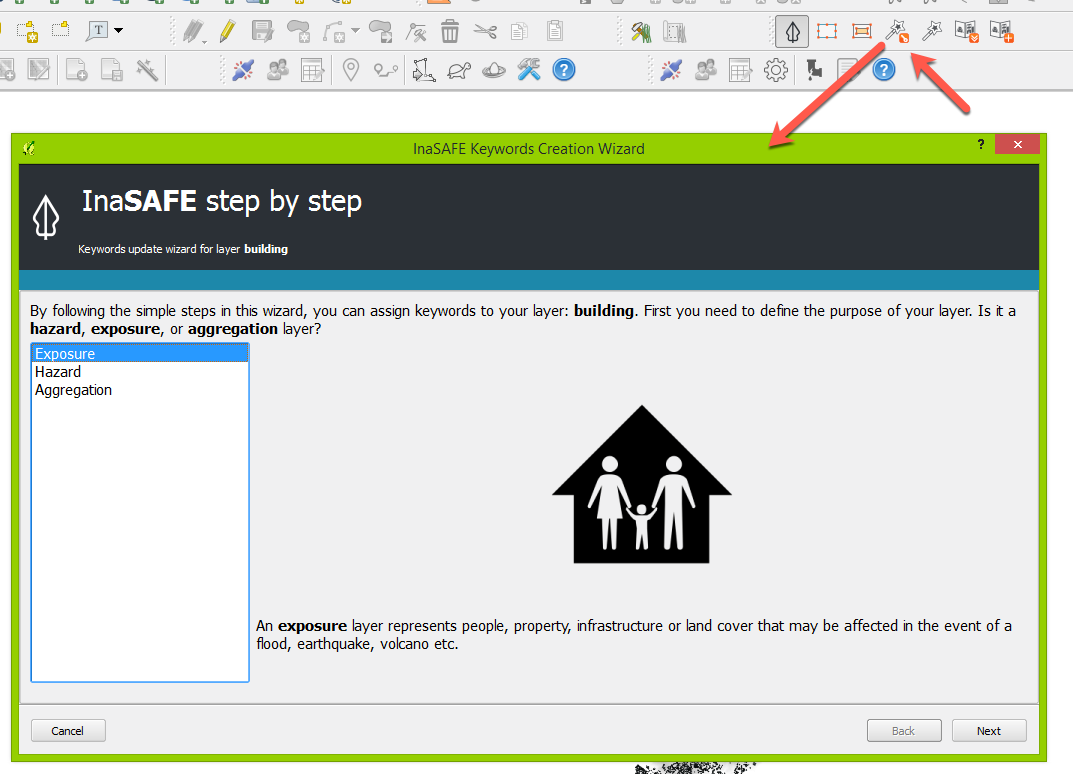
\includegraphics[width=9cm]{Images/keyword1.png}
	\caption{Declaring building layer as Exposure dataset}\label{fig:keyword1}
\end{figure}

\begin{figure}[htb]
	\centering
	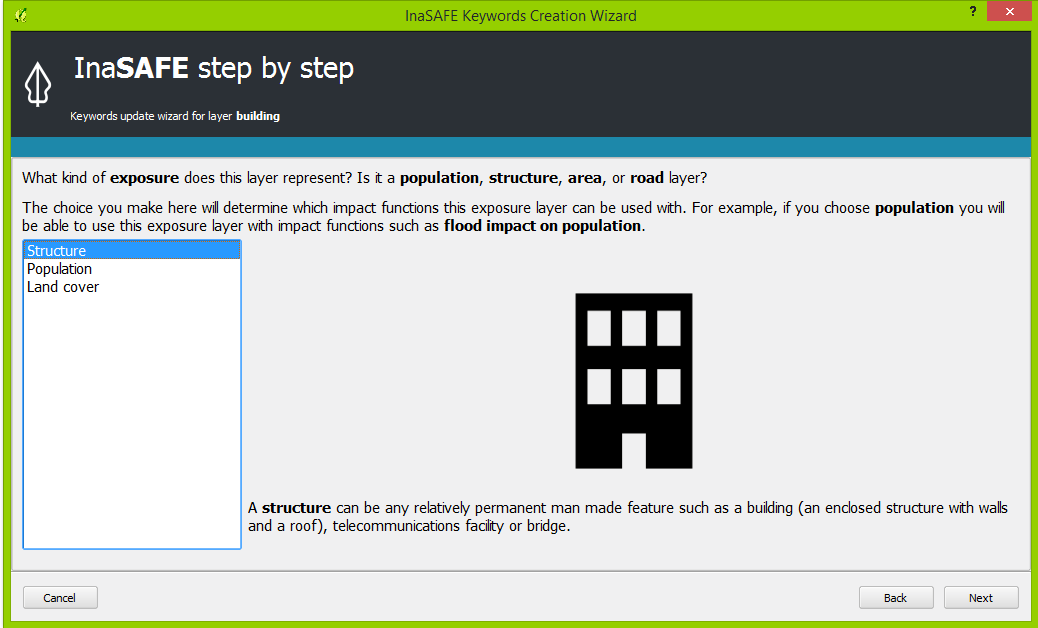
\includegraphics[width=9cm]{Images/keyword2.png}
	\caption{Assigning \textit{Structure} keyword to building layer}\label{fig:keyword2}
\end{figure}

\begin{figure}[htb]
	\centering
	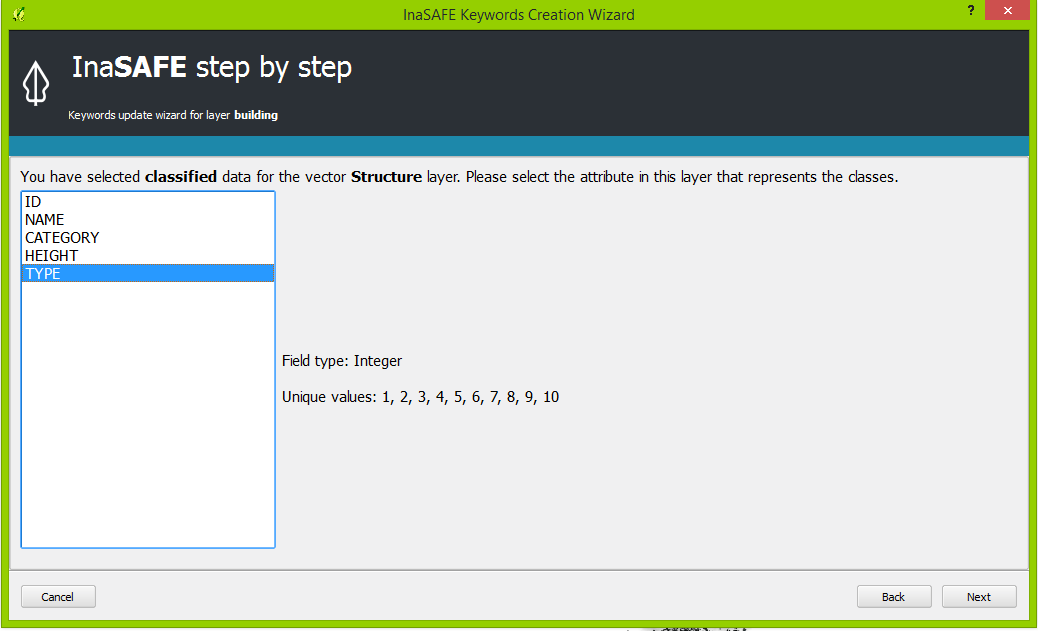
\includegraphics[width=9cm]{Images/keyword3.png}
	\caption{Selecting the attribute defining the building type}\label{fig:keyword3}
\end{figure}

Assign the numeric type values to the structure classes defined in InaSAFE by dragging the numeric values and dropping them on the structure classes (Figure \ref{fig:keyword4}). Click \textit{Next} until you reach the end of the \textit{Keyword Creation Wizard}.

\begin{figure}[htb]
	\centering
	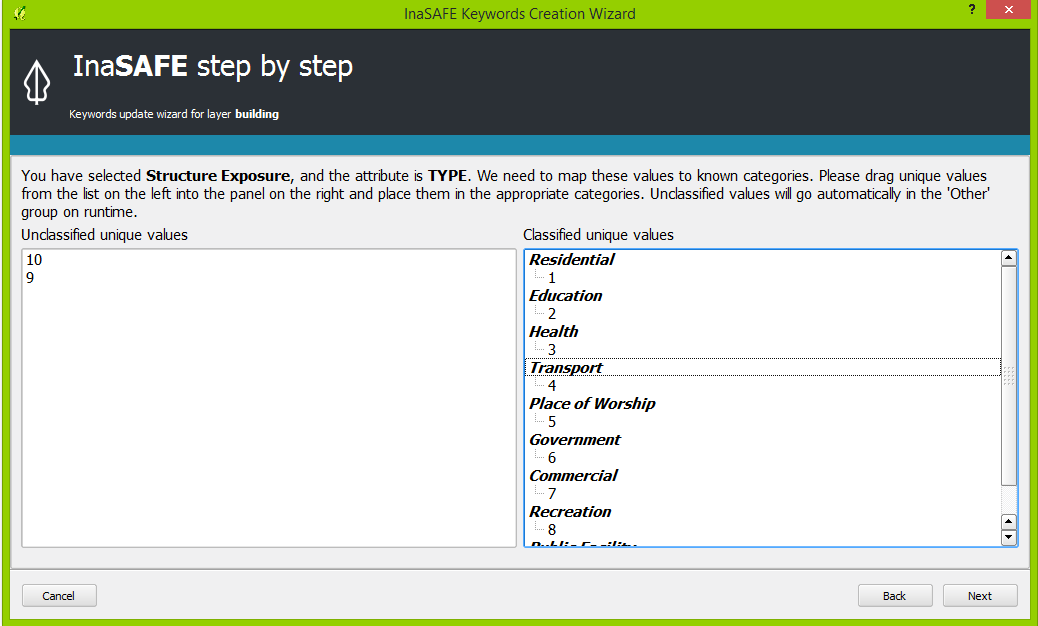
\includegraphics[width=9cm]{Images/keyword4.png}
	\caption{Relating codes to structure classes}\label{fig:keyword4}
\end{figure}

Repeat the same steps for the \textit{road} layer and select the \textit{CATEGORY} attribute this time as the one containing the road classes.

\subsection{Hazard layer}

Select the \textit{inundation\_final} layer in the table of contents and run the \textit{Keyword Creation Wizard}. Select \textit{Hazard} in the first step and \textit{Tsunami} in the second. Select \textit{Single event} in the third step and \textit{Continuous} in the forth one. Select \textit{Metres} as the unit for the inundation data. Click \textit{Next} until you reach the end of the \textit{Keyword Creation Wizard}.

\subsection{Aggregation layer}

Select the \textit{district} layer in the table of contents and run the \textit{Keyword Creation Wizard}. Select \textit{Aggregation} in the first step and \textit{NAME} as the attribute containing the names of the aggregation areas in the second step.Click \textit{Next} until you reach the end of the \textit{Keyword Creation Wizard}.

\section{Performing impact analyses}

\subsection{Identifying extent and level of the impact}

Everything done so far was just preparation work for the actual impact analyses. Once the keywords are assigned to the datasets InaSAFE will offer the various analyses possible through its \textit{Question} form (Figure \ref{fig:analysis1}). 

\begin{figure}[htb]
	\centering
	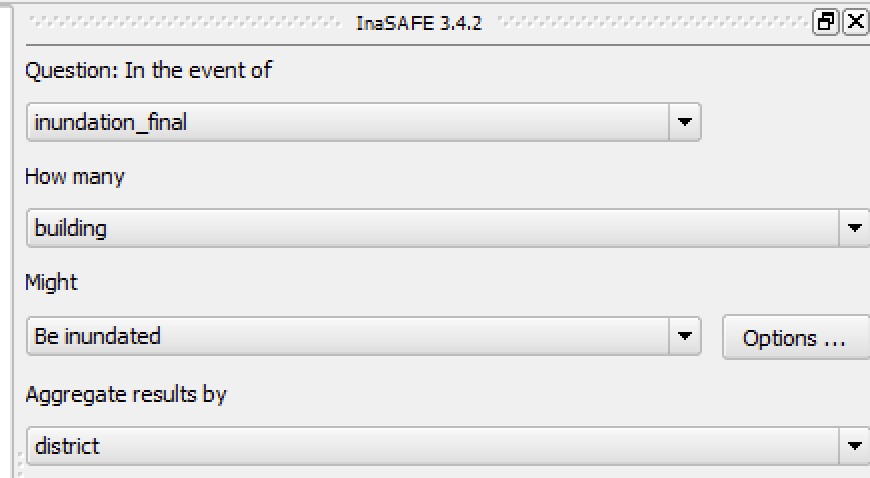
\includegraphics[width=7cm]{Images/analysis1.png}
	\caption{Question form listing the available analyses}\label{fig:analysis1}
\end{figure}

Run the first analysis (``Impact Function'' in the InaSAFE terminology) to identify the structures/buildings affected by inundation by clicking the \textit{Run} button. Depending on your laptop's performance the analysis can take quite some time. Eventually a new layer will be added to the table of contents and a report be shown in the InaSAFE dock widget (Figure \ref{fig:analysis2}). The layer shows the buildings categorised by level of inundation. The result in numbers is shown in the report.

\begin{figure}[htb]
	\centering
	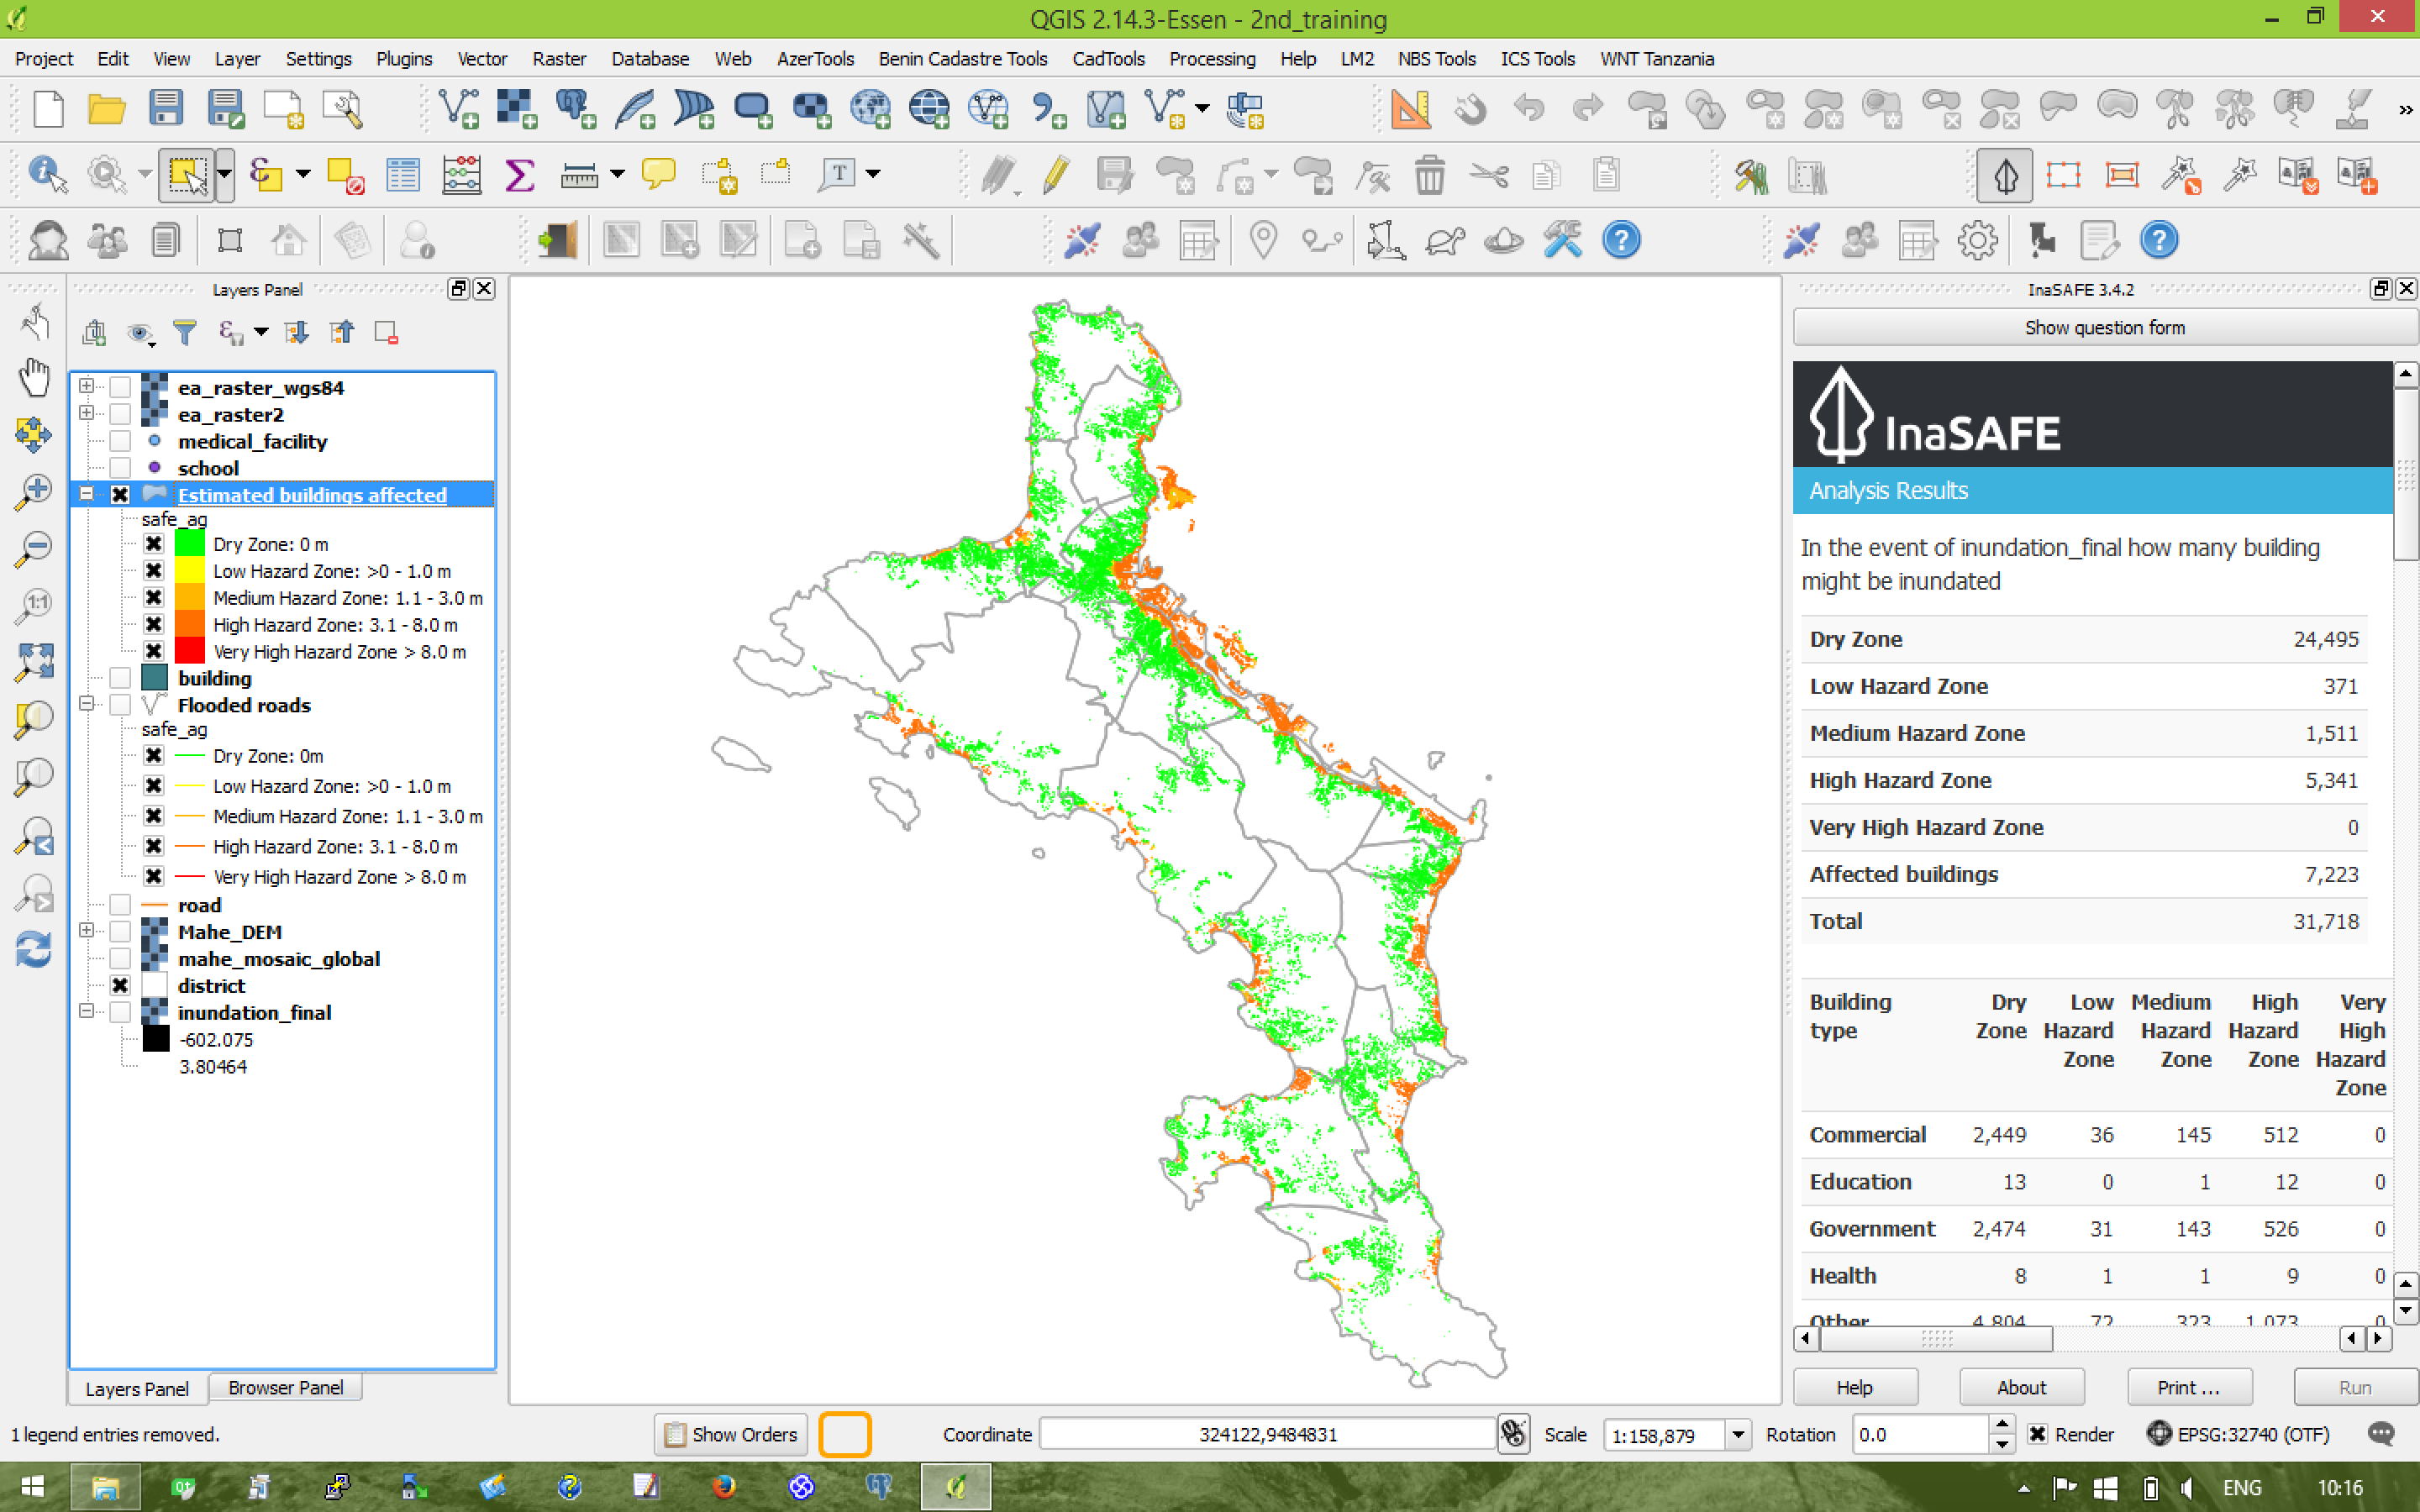
\includegraphics[width=12cm]{Images/analysis2.png}
	\caption{Impact analysis results for buildings}\label{fig:analysis2}
\end{figure}

Check map and report to verify whether the results are credible.
You will find buildings on Cerf Island classified as \textit{Dry}. This is wrong. But for Cerf Island no inundation data was available and thus, InaSAFE just classified the buildings as \textit{Dry}. To avoid such misclassification it is a good idea to delete buildings that are not covered by the inundation layer before performing the impact analysis. Just do that and repeat the analysis. Finally you can print the results to a PDF file by clicking the \textit{Print} button on the InaSAFE dock widget. The \textit{Print} button is enabled only when the result layer is selected in the table of contents. When printing you can select from several print templates. An appropriate one for your results would be \textit{a3-portrait-orange} for example. This print could now be used by the authorities in charge to prepare evacuation measures and provision of support accordingly. 

Run the second analysis to identify the roads affected by inundation (Figure \ref{fig:analysis3}). Although there are significantly less road features than building features the analysis takes considerable longer for some reason. Grab a cup of coffee meanwhile. Once the analysis has been completed verify that the results make sense.

\begin{figure}[htb]
	\centering
	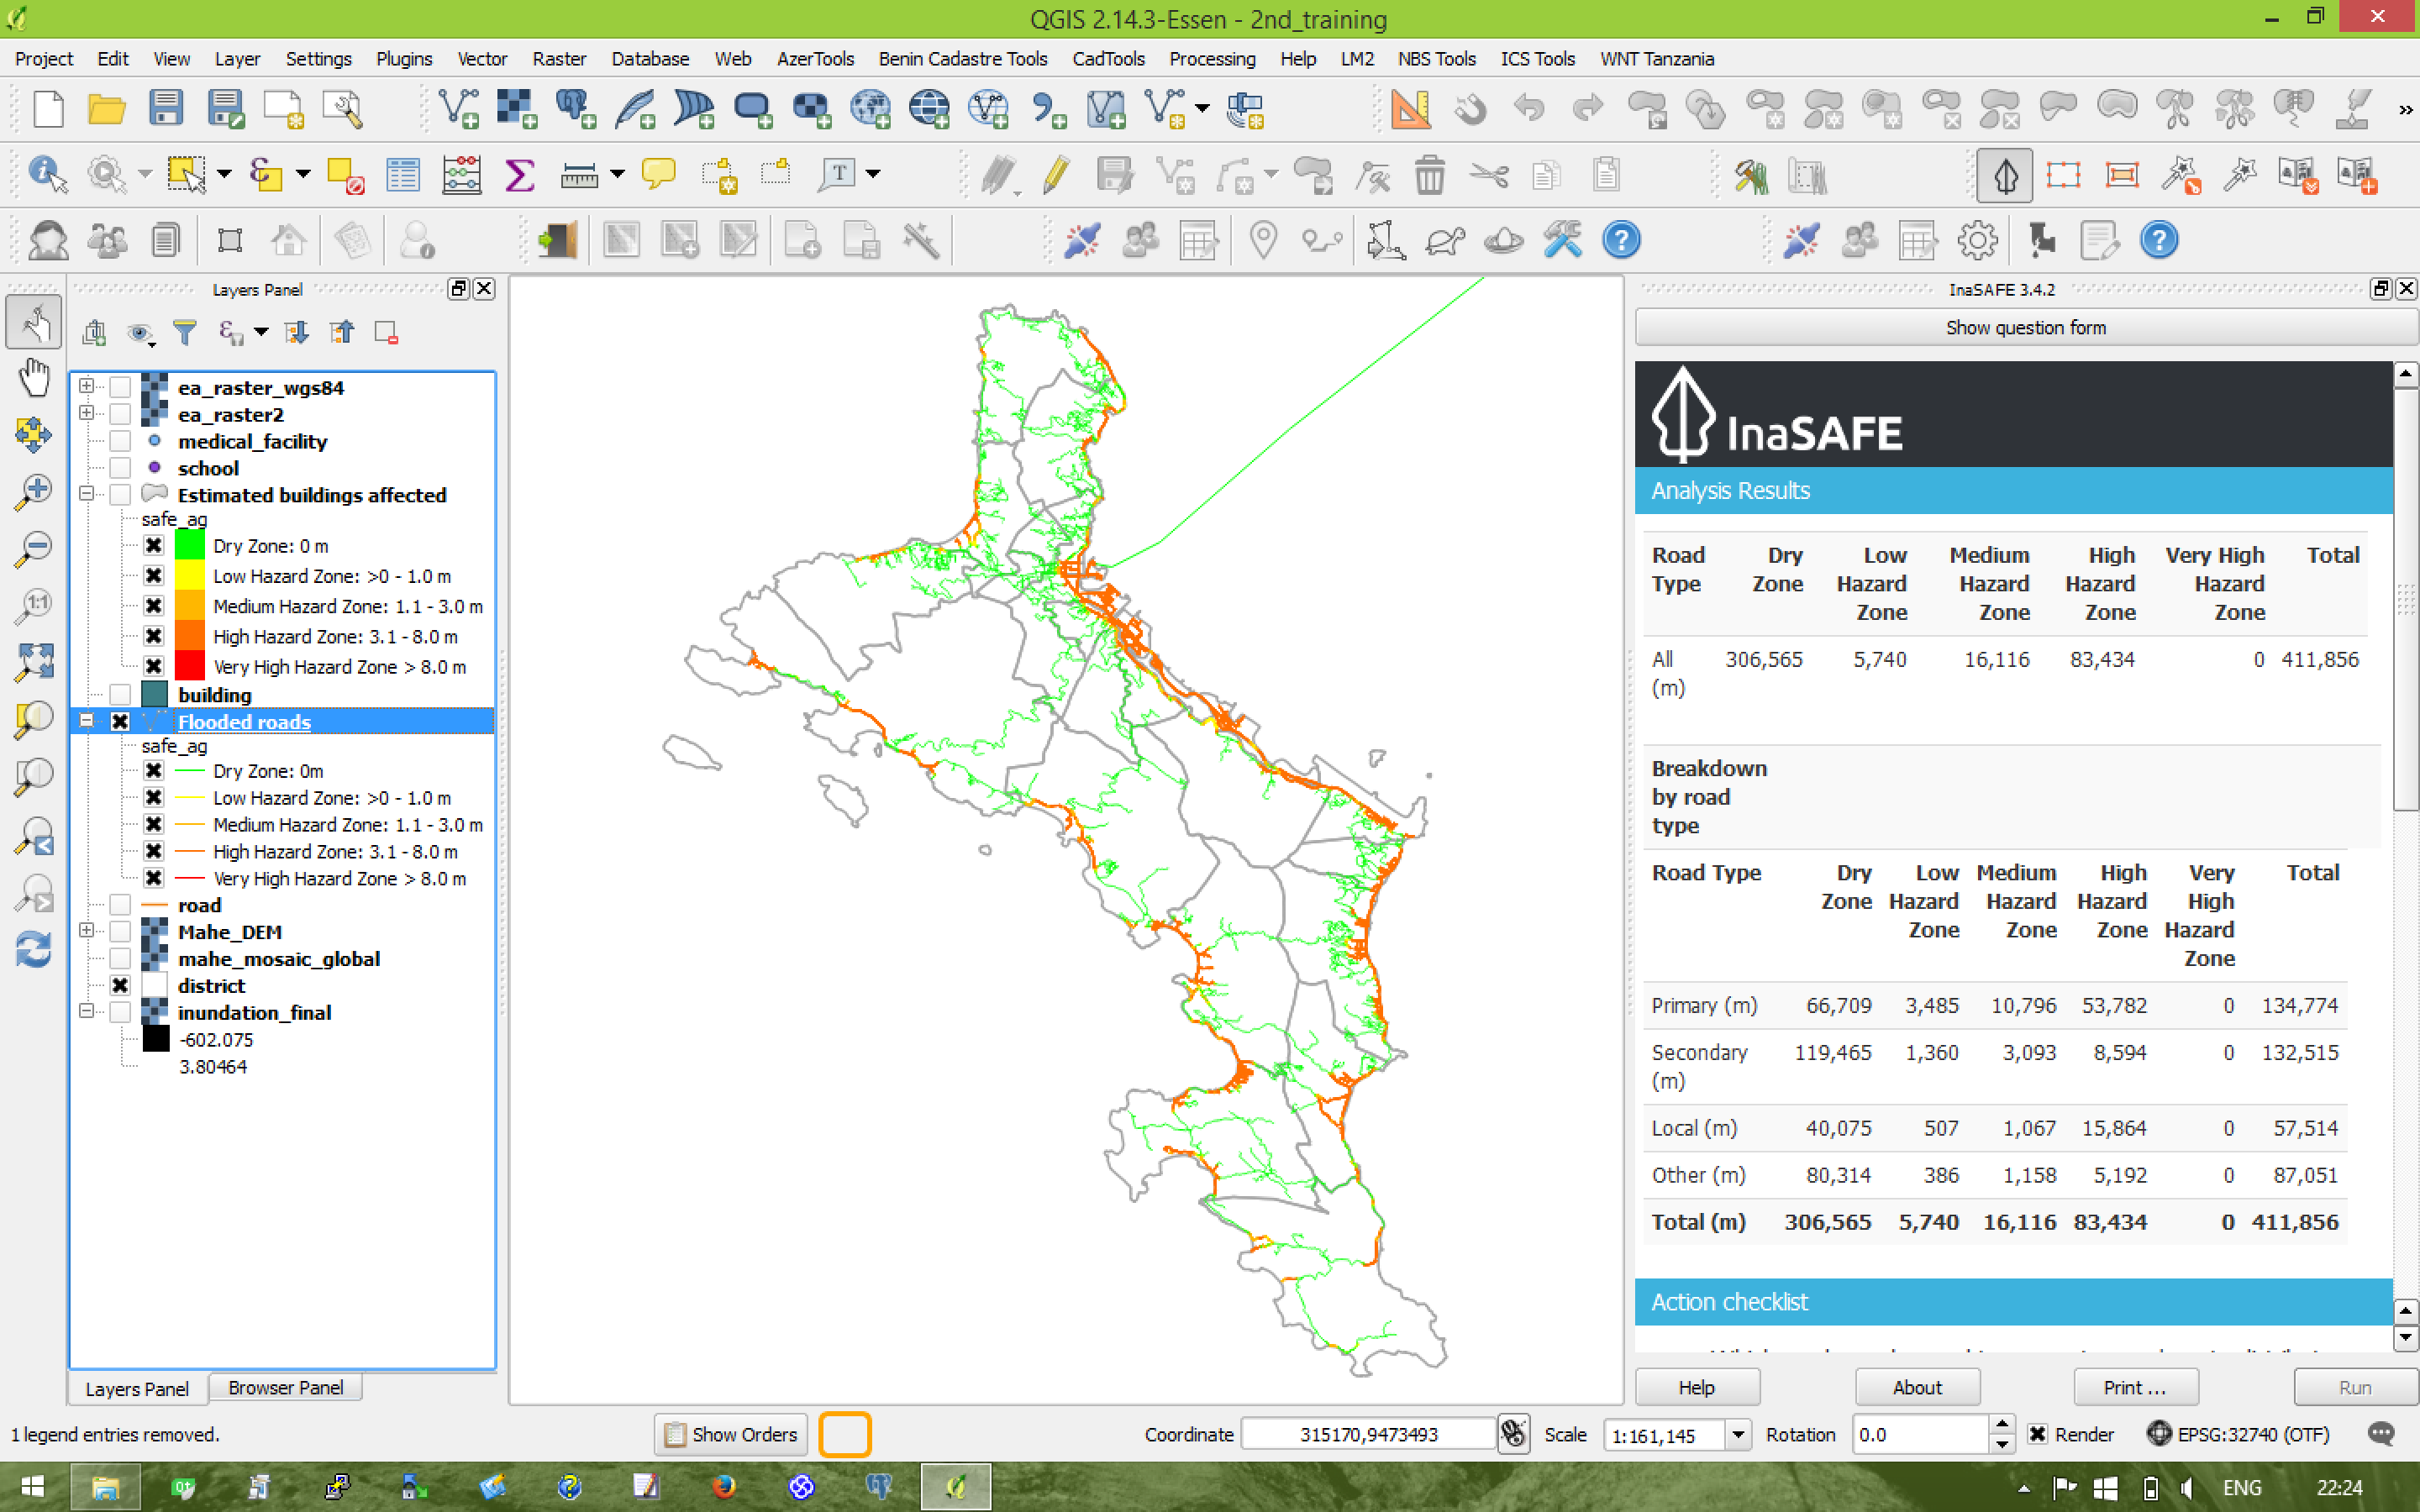
\includegraphics[width=12cm]{Images/analysis3.png}
	\caption{Impact analysis results for roads}\label{fig:analysis3}
\end{figure}

For each impact function you can modify the configuration, usually to change some threshold values applied to the classification. Click the \textit{Options} button in the \textit{Question} form to open the \textit{Configuration} dialog. In case of the impact function \textit{Tsunami on buildings} it is the thresholds for the inundation levels that are used to identify the hazard levels (Figure \ref{fig:analysis4}). Change the threshold values and re-run the analysis.

\begin{figure}[htb]
	\centering
	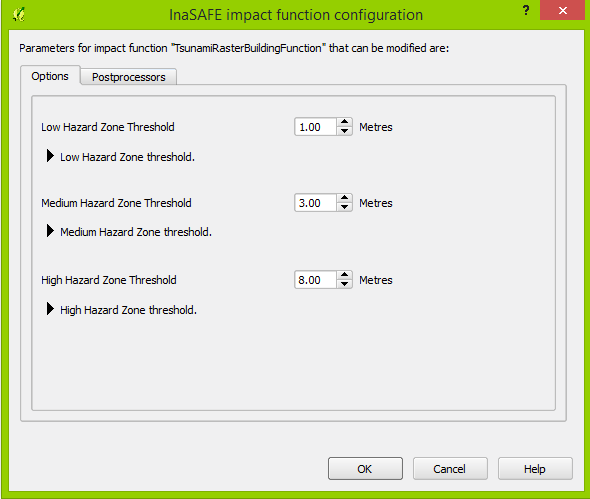
\includegraphics[width=8cm]{Images/analysis4.png}
	\caption{Changing threshold values of impact function}\label{fig:analysis4}
\end{figure}

\subsection{Damage and loss assessment}

Damage is commonly calculated as the replacement value of totally or partially destroyed physical assets. Loss on the other hand results from interrupted flows of economy caused by the temporary absence of damaged assets. Calculating loss is a lot more complex than calculating damage since numerous aspects play a role in loss assessment. Because of this the exercise will focus on damage assessment.

Open the file \textit{ReplacementValues.xslx} from the \textit{Data/ReplacementValues} folder. The file was provided by a quantity surveyor of the \gls{mluh} and contains the replacement costs for many of the structure types. In this exercise we will focus on the damage of residential, health care and education relating buildings. You can see that the categories in the Excel file are a lot more detailed than the categories/types of buildings in the \textit{building} layer. Thus, based on the Excel sheet we will just assume the base values as follows:

\begin{itemize}
	\item Residential: 9,000 SCR/sqm
	\item Health: 14,000 SCR/sqm
	\item Education: 13,000 SCR/sqm
\end{itemize}

Based on the level of hazard the following factors shall be applied:

\begin{itemize}
	\item Low: 10\%
	\item Medium: 50\%
	\item High/Very High: 100\%
\end{itemize}

With these assumptions you can now use the \textit{Field Calculator} and calculate the damage for each building in the result layer of your InaSAFE analysis. Based on the numeric codes you assigned for your building categories you will need to do an attribute query first to select residential buildings only. Then use the \textit{Field Calculator} as shown in Figure \ref{fig:calc_damage}.

\begin{figure}[htb]
	\centering
	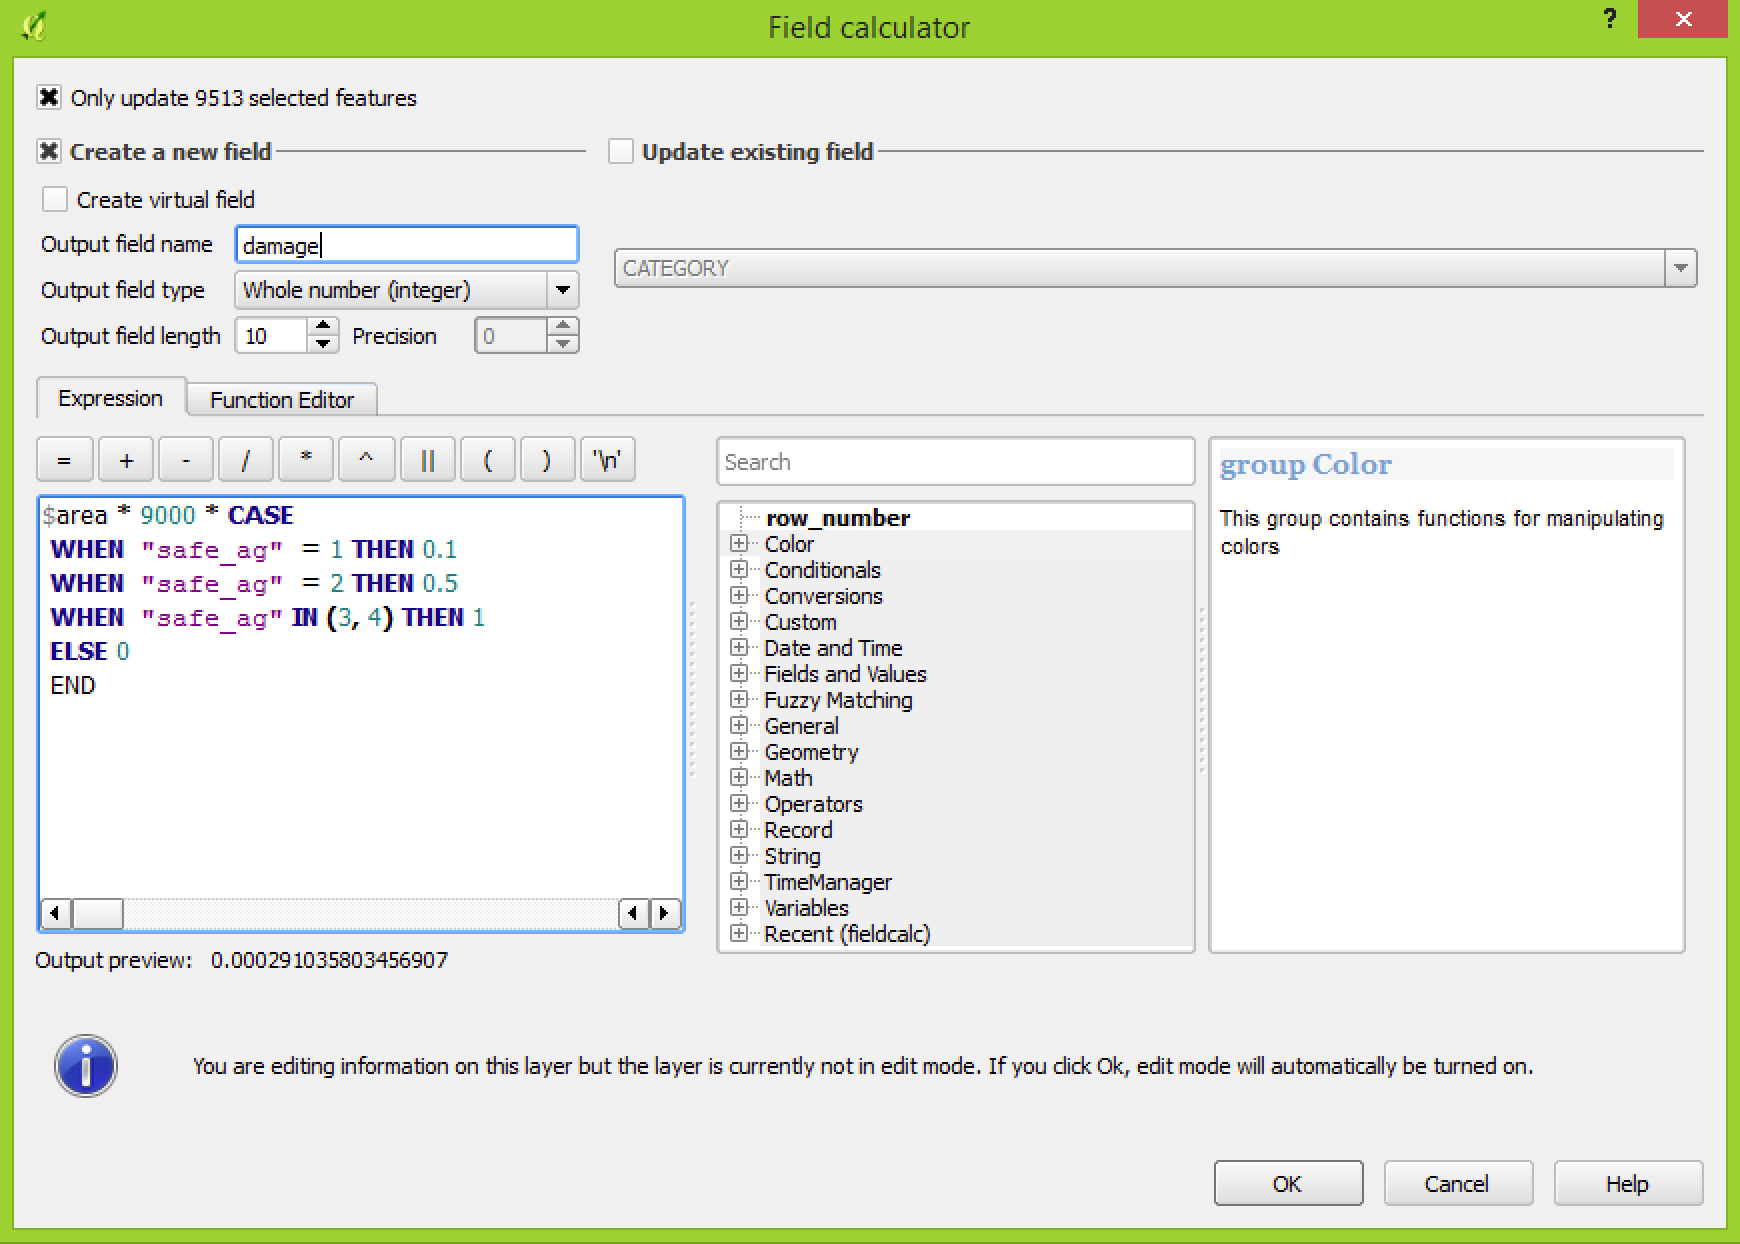
\includegraphics[width=8cm]{Images/calc_damage.png}
	\caption{Formula to calculate damage of residential buildings}\label{fig:calc_damage}
\end{figure}

The \textit{safe\_ag} field created by InaSAFE is used to apply the correct factor depending on the hazard (and damage) level.

Repeat the same steps for the health care and education buildings but select \textit{Update existing field} in the \textit{Field Calculator} since the \textit{damage} field has already been created. Don't forget to adjust the base value in the formula. Finally select all remaining buildings (where \textit{damage} IS NULL) and set the \textit{damage} field to 0 (instead of NULL). This avoids issues when calculating statistics later on.

\begin{figure}[htb]
	\centering
	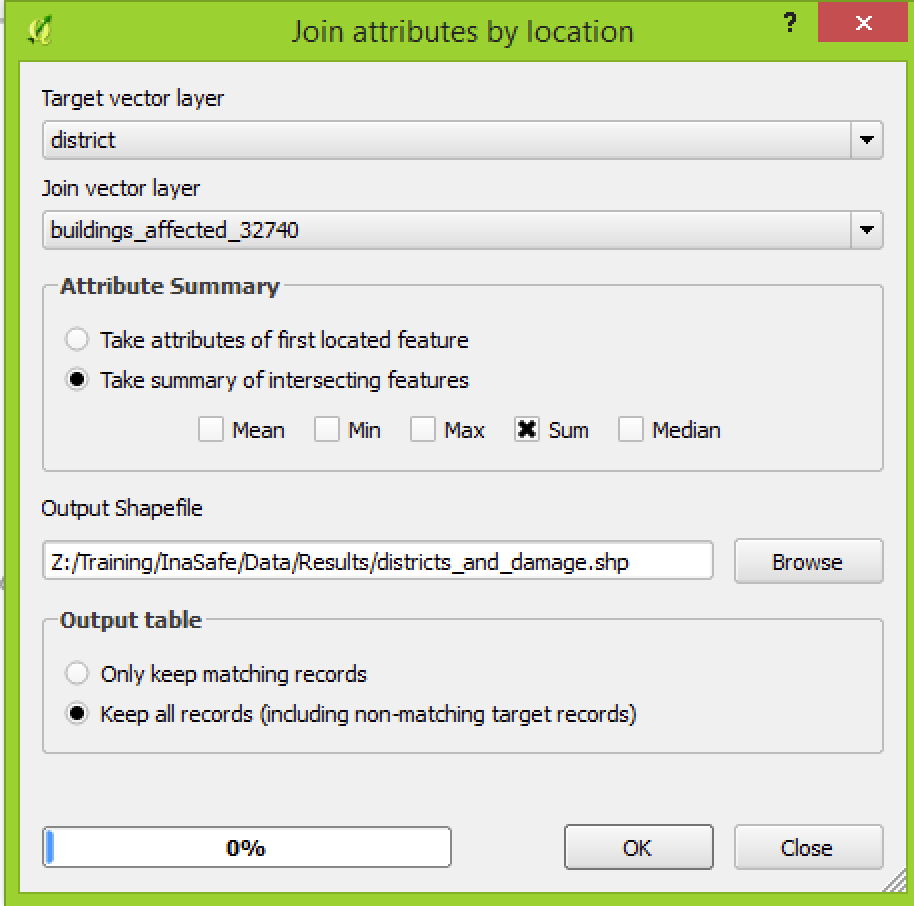
\includegraphics[width=8cm]{Images/spatial_join.png}
	\caption{Performing a spatial join}\label{fig:spatial_join}
\end{figure}

Now let's aggregate the damages per district to show how much each district is affected in terms of damage. You will use a spatial join to aggregate (sum) the damage values of the buildings and assign them to the districts. For the spatial join to work both layers (districts and affected buildings) have to have the same coordinate reference system. InaSAFE creates its result layers in WGS84 (EPSG:4326) while all your original Shapefile layers are in EPSG:32740. Thus, save the \textit{Estimated buildings affected} layer to a new Shapefile with coordinate reference system EPSG:32740 and name it \textit{buildings\_affected\_32740}. From menu \textit{Vector:Data Management Tools} select the \textit{Join Attributes by Location} tool. Apply the settings as shown in Figure \ref{fig:spatial_join}. As a last step create a thematic map showing the districts by amount of damage. Your result might look  similar to Figure \ref{fig:districts_by_damage}.

\begin{figure}[htb]
	\centering
	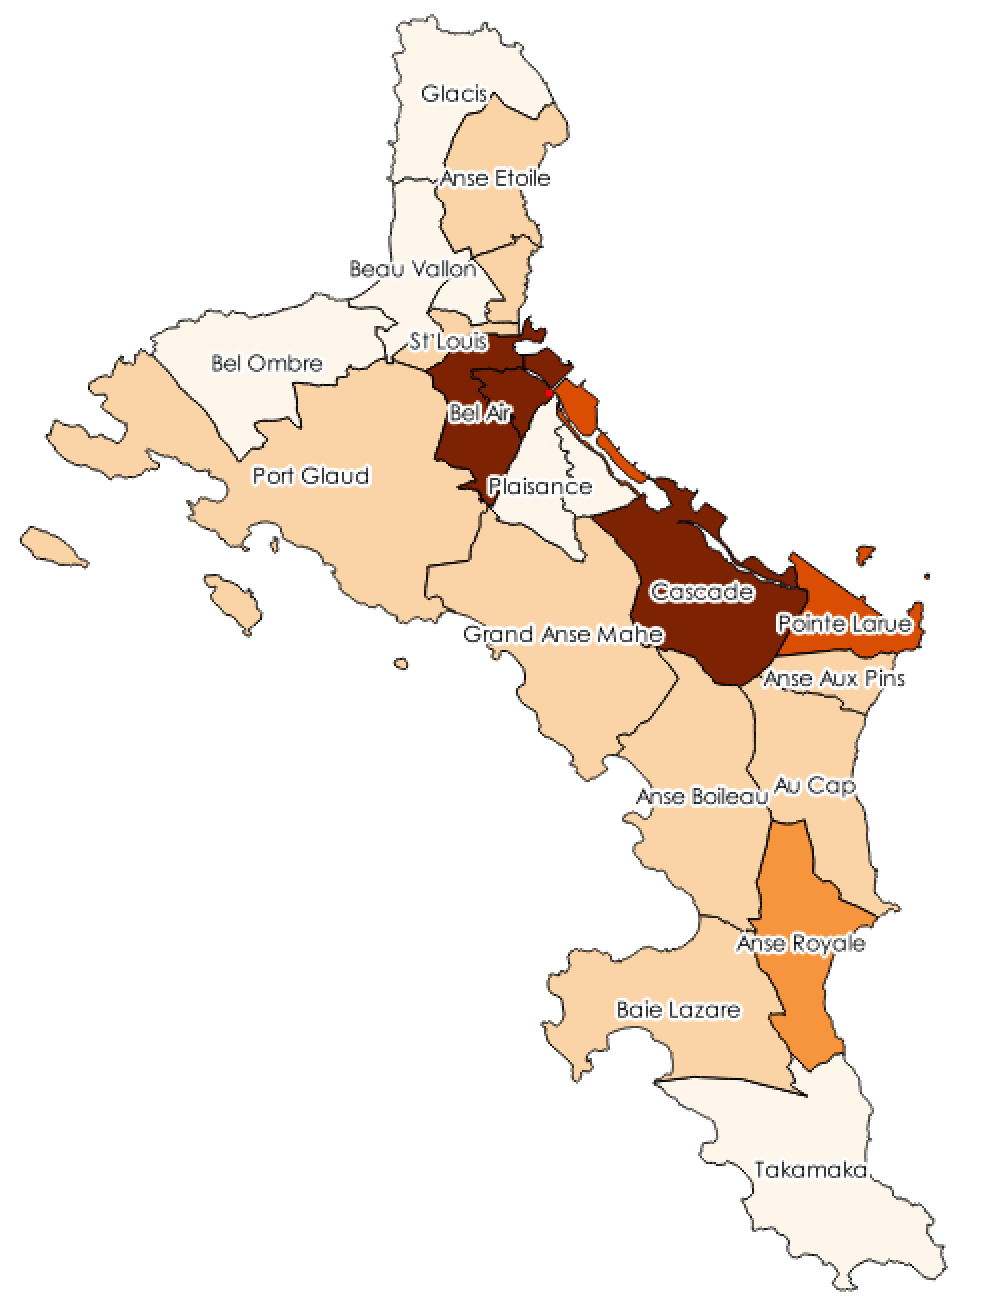
\includegraphics[width=8cm]{Images/districts_by_damage.png}
	\caption{Districts by damage}\label{fig:districts_by_damage}
\end{figure}



\end{document}
